\documentclass[a4paper, 12pt]{article}
%\usepackage[T1]{fontenc}
\usepackage[left=2cm,right=2cm,top=2cm,bottom=2cm,includeheadfoot]{geometry}
\usepackage[utf8]{inputenc}
\usepackage[ngerman]{babel}
\usepackage{enumitem}
\usepackage{pdfpages}
\usepackage{ulem} 
\usepackage{graphicx}
\usepackage{caption}
\usepackage{subcaption}
\usepackage{listings}
\usepackage{verbatim}
\usepackage{fancyhdr}
\usepackage{hyperref}
\lstset{
	language=c++,
	extendedchars=\true,
	inputencoding=utf8,
	basicstyle=\ttfamily\footnotesize,
	identifierstyle=,
	stringstyle=\ttfamily\small, 
	showstringspaces=false,
	commentstyle=\color{codegreen},
	keywordstyle=\color{blue},
	stringstyle=\color{codegray}, 
	breakatwhitespace=false,         
	breaklines=true, 
	captionpos=b,                    
	keepspaces=true,                 
	numbers=left,                    
	numbersep=5pt,                  
	showspaces=false,                
	showstringspaces=false,
	showtabs=false,                  
	tabsize=2,
	aboveskip=1em,
}
\usepackage{color}
\usepackage{comment}
\usepackage{todonotes}


\definecolor{codegreen}{rgb}{0,0.6,0}
\definecolor{codegray}{rgb}{0.5,0.5,0.5}
%\definecolor{backcolour}{rgb}{0.95,0.95,0.92}

\pagestyle{fancy}
\lhead[Sascha Beyer, David Schneebauer]{Sascha Beyer, David Schneebauer}
\chead[Projektarbeit Hurace]{Projektarbeit Hurace}
\rhead[SWK5 GRP1 SEBakk BB WS18-19]{SWK5 GRP1 SEBakk BB WS18-19}

%opening
\title{Projektarbeit Hurace}
\author{Sascha Beyer, David Schneebauer}
\date{\today{}, Hagenberg}

\begin{document}
	\maketitle
	\tableofcontents
	\newpage
	\section{Installationsanleitung}
	
	\begin{enumerate}
		\item{Sourcecode von GitHub clonen (https://github.com/swk5-2019ws/bb-hurace-g1-beyer-g1-schneebauer.git)}
		\item{Die Solution Hurace.sln mit Visual Studio oder Rider öffnen}
		\item{RaceControl und / oder Api als Projekt starten}
		\item{Die Datenbank wird automatisch mit den entsprechenden Daten befüllt und gestartet}
		\item{Die Api bzw. das RaceControl kann verwendet werden}
	\end{enumerate}
	
	

	\section{Hurace.Core}
	\subsection{DAL}
	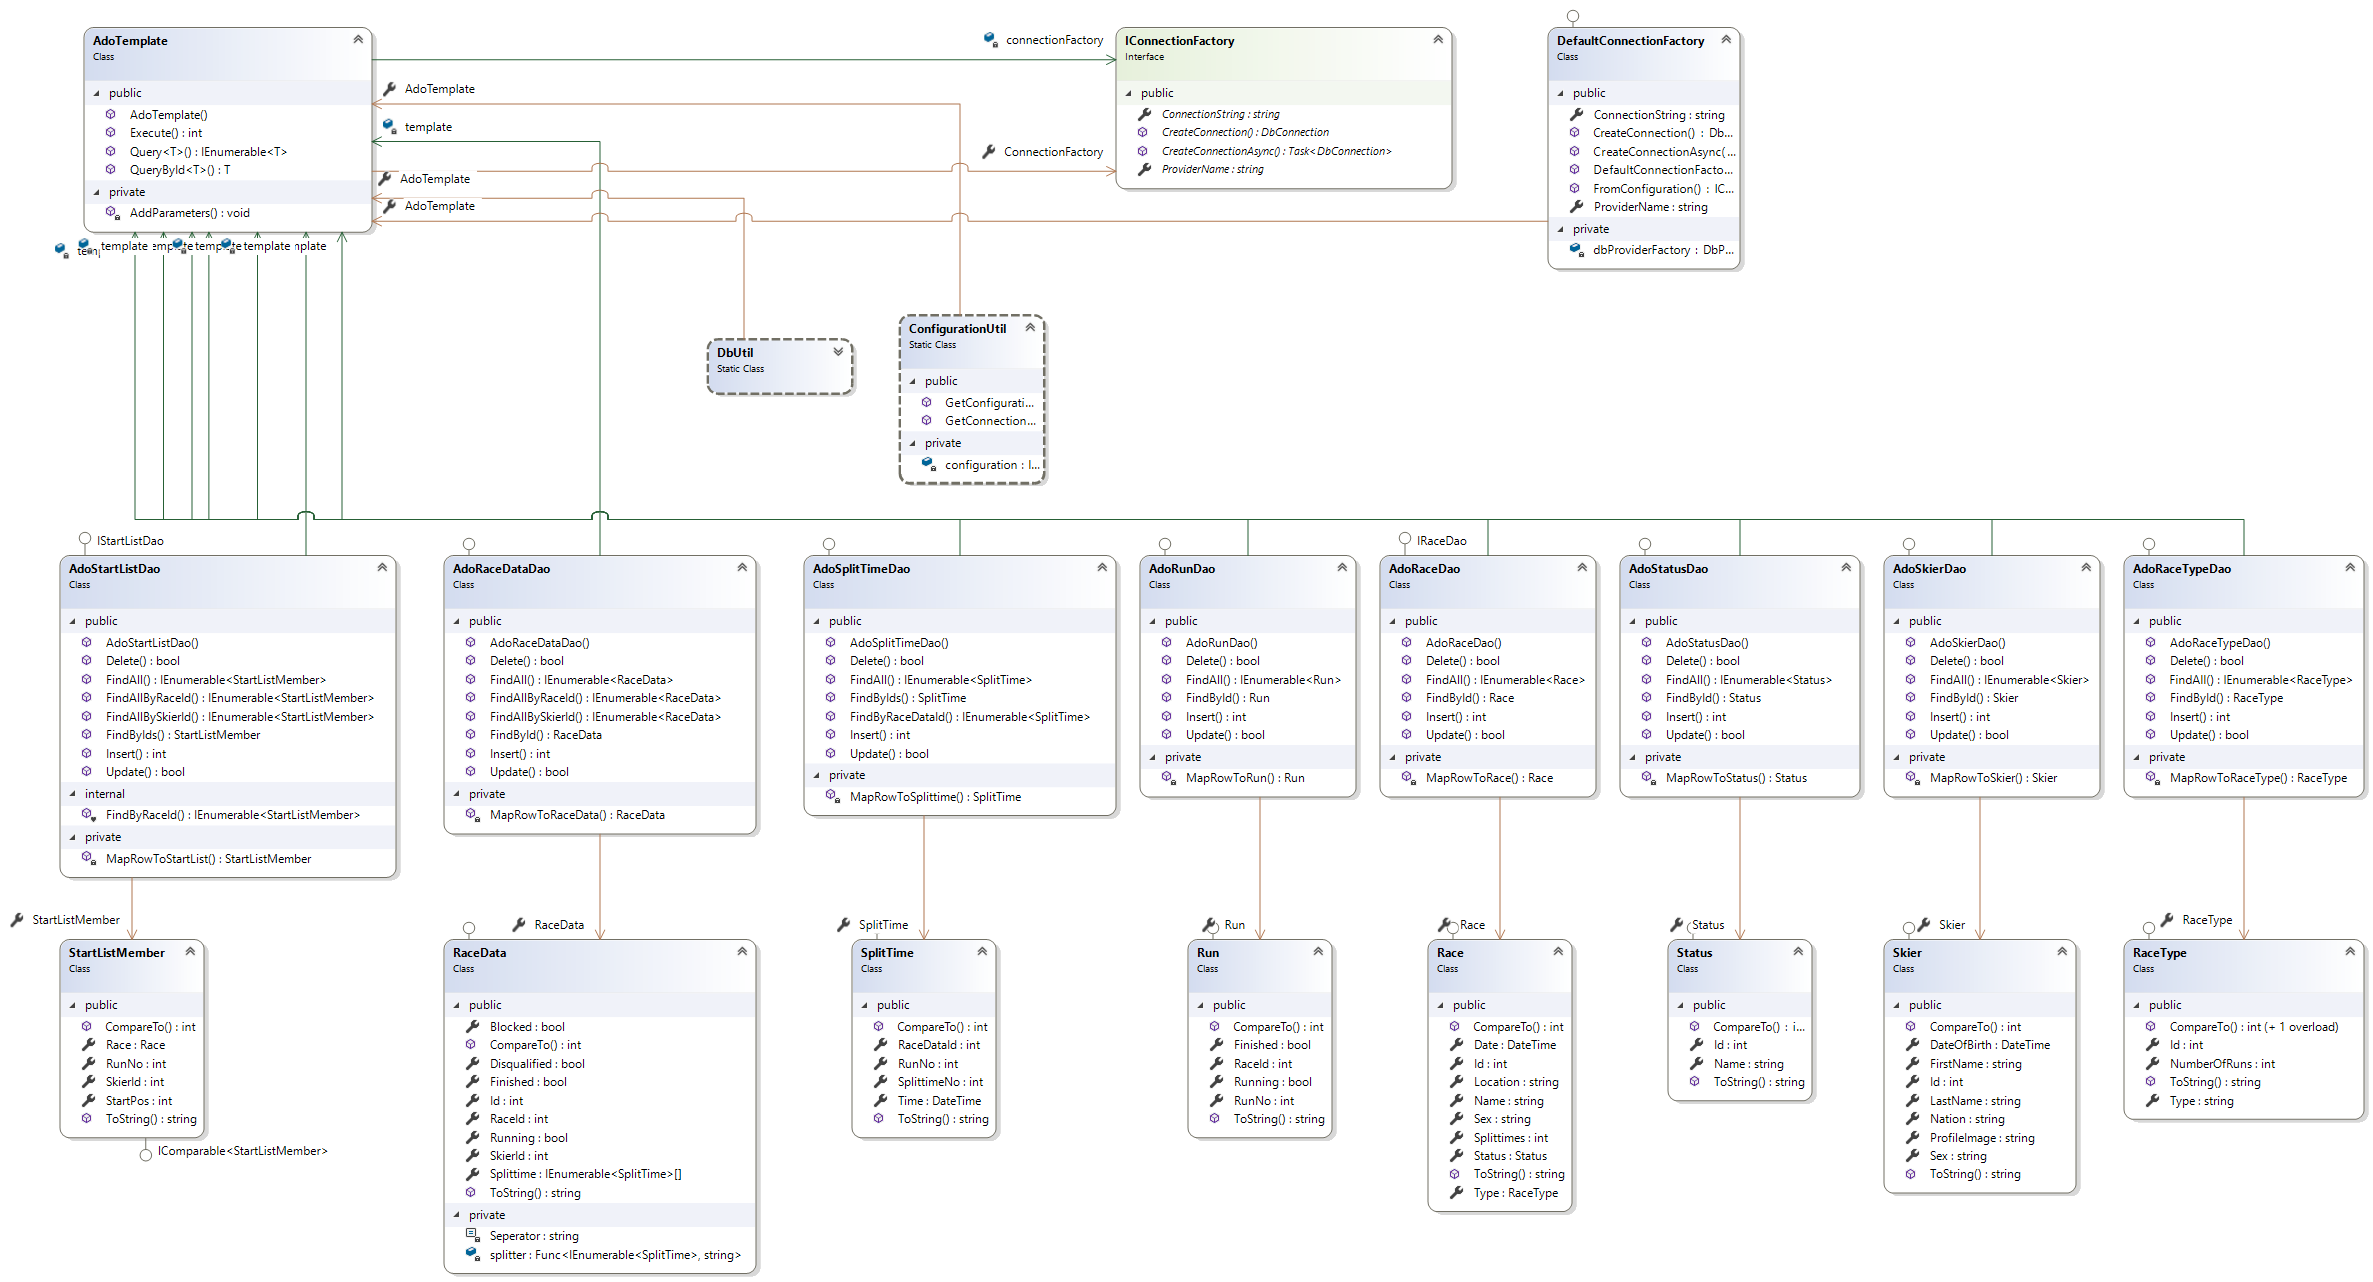
\includegraphics[width=.9\textwidth]{img/DAL.png}
	\subsubsection{Datenbankmodell}
	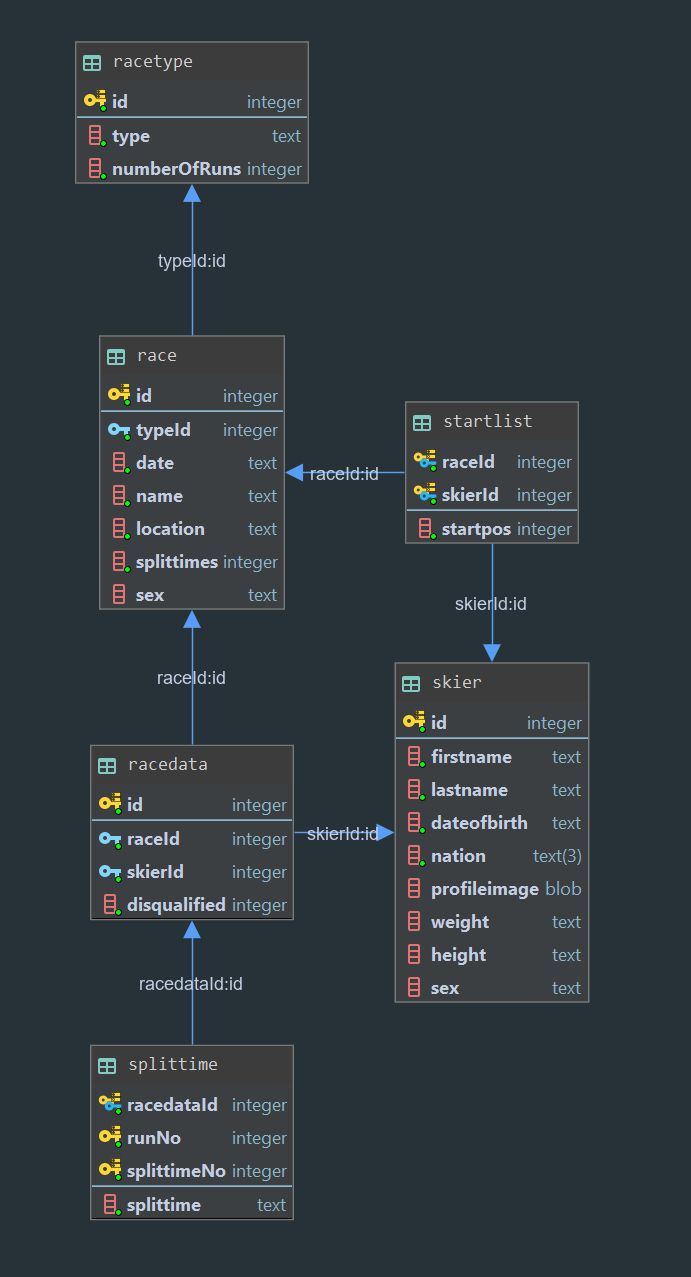
\includegraphics[width=.5\textwidth]{img/huraceDB.png}
	%\lstinputlisting[language=Java]{../Dal/Interface/IRaceDao.cs}
	%\newpage
	%\lstinputlisting[language=Java]{../src/queues/DHeapQueue.java}
	%\newpage
	\newpage
	\subsubsection{Datenbankzugriffsschicht}
	Zur Persistierung der Daten wird eine SQLite Datenbank verwendet. Zur Herstellung der Verbindung wird das Factory Pattern verwendet. Über eine Konfigurationsdatei werden Informationen zum Datenbanktyp zur Verfügung gestellt. Für jede Entität sind DAO Klassen implementiert. Diese stellen Methoden für Operationen auf der Datenbank zur Verfügung. Um generisch zu bleiben wird gegen Interfaces implementiert.
	\newline
	 
	\textbf{ISkierDao}
	\lstinputlisting[language=c++]{../Core.Dal/Interface/ISkierDao.cs}
	\textbf{AdoSkierDao}
	\lstinputlisting[language=c++]{../Core.Dal/Ado/AdoSkierDao.cs}
	
	Die DAO Klassen instanzieren ein Ado-Template welches die Datenbank Operationen generisch regelt.
	
	\textbf{AdoTemplate}
	\lstinputlisting[language=c++]{../Core.Dal/Common/AdoTemplate.cs}
	
	Um mit schlüssigen Daten arbeiten zu können, bevor der Simulator fertig implementiert ist, wurden Importer geschrieben die diese generieren und in der Datenbank speichern.
	
	\subsection{Logic}
	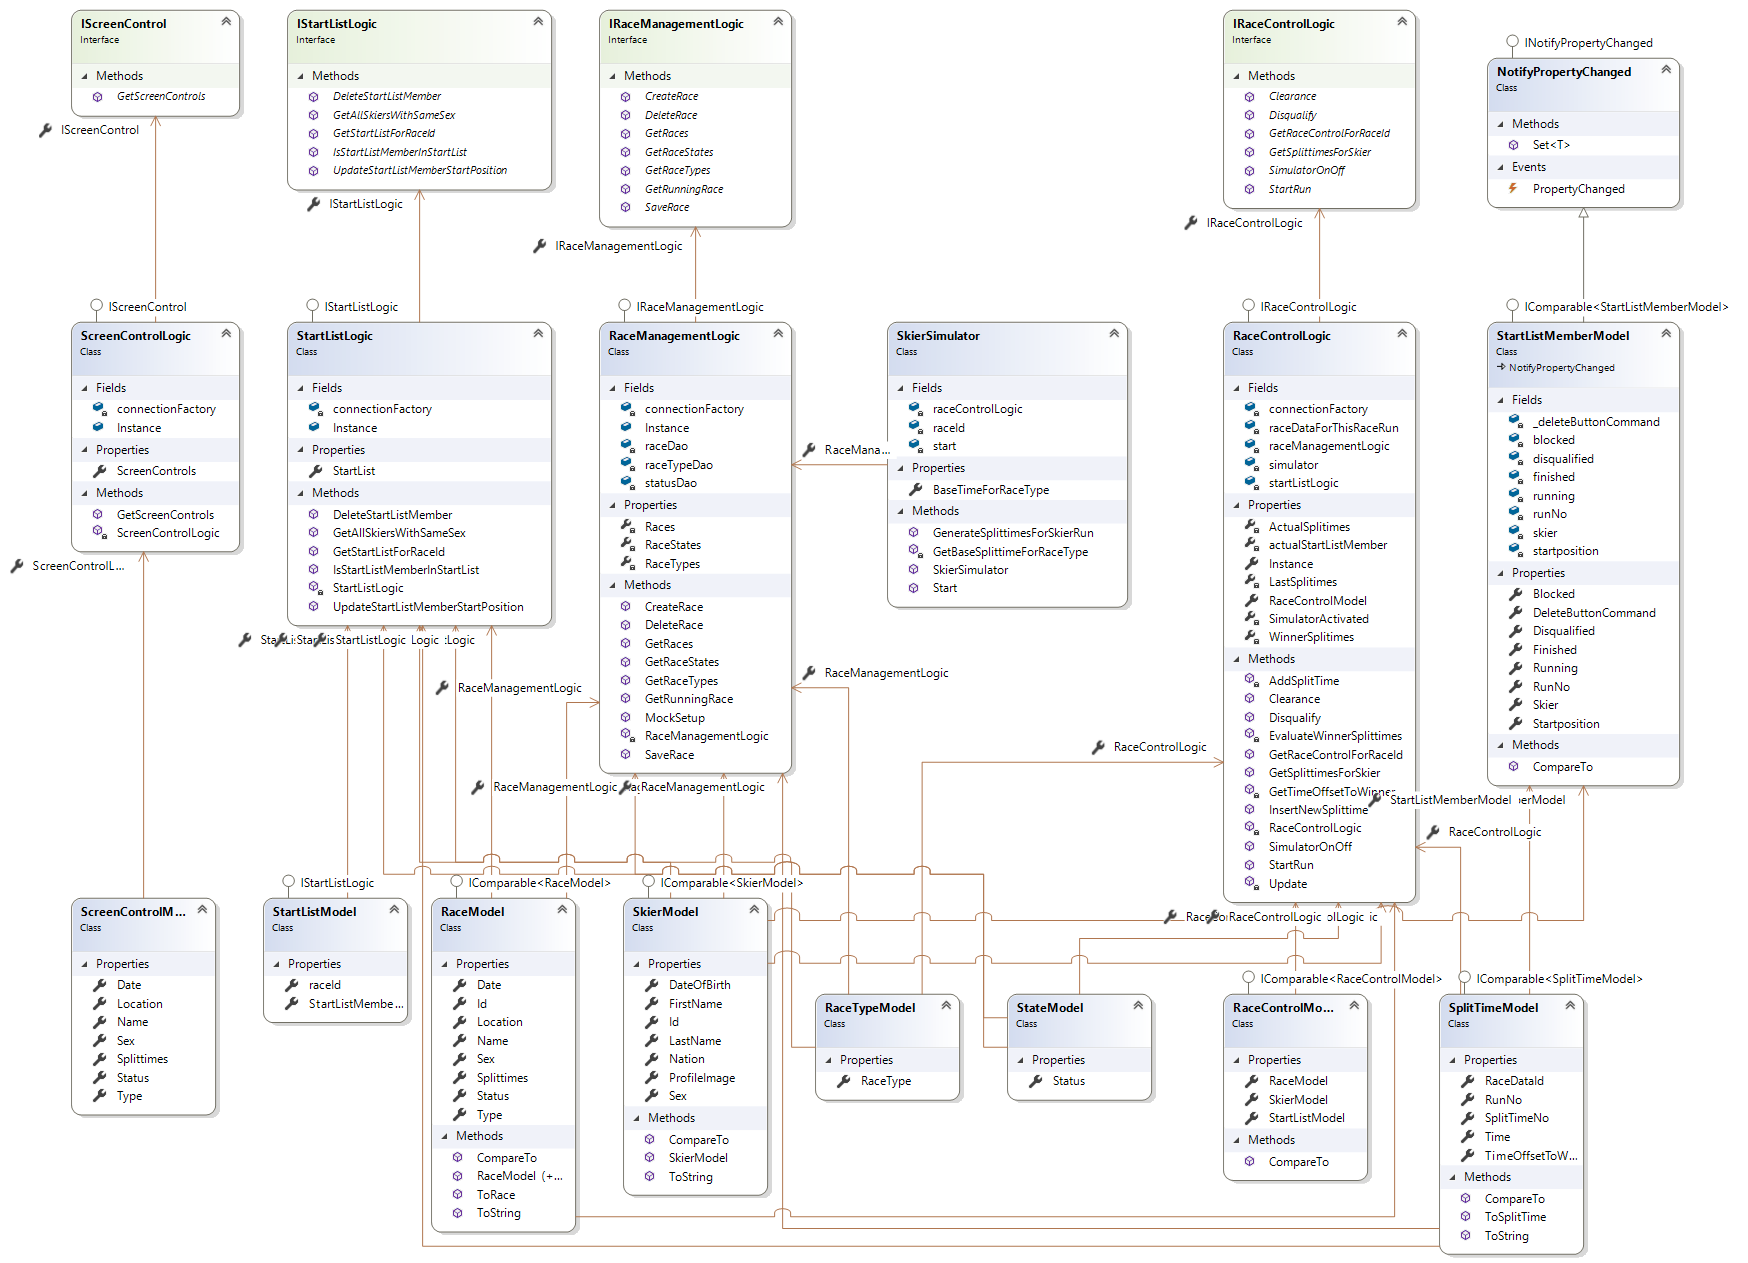
\includegraphics[width=.9\textwidth]{img/Logic.png}\\
	
	\subsection{Wiederaufsetzen}
	Nachdem die Werte in der Datenbank persistiert werden kann ein Neustart der Anwendung leicht erfolgen ohne den Status zu verlieren.
	
	\subsection{Abfragen}
	Für jegliche Abfragen der Clients, ist eine wie oben dargestellte Dao Klasse mit entsprechenden Methoden definiert. Mögliche weitere Anpassungen an den Ergebnissen werden im Client durchgeführt.
	
	\subsection{UnitTests}
	Die entsprechenden DAO Klassen wurden zusammen mit der restlichen Datenbankzugriffsschicht getestet. 
	\newline
	\newline
	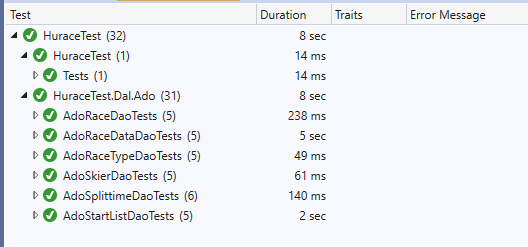
\includegraphics[width=.7\textwidth]{img/UnitTests.png}
	
	\section{Hurace.RaceControl}
	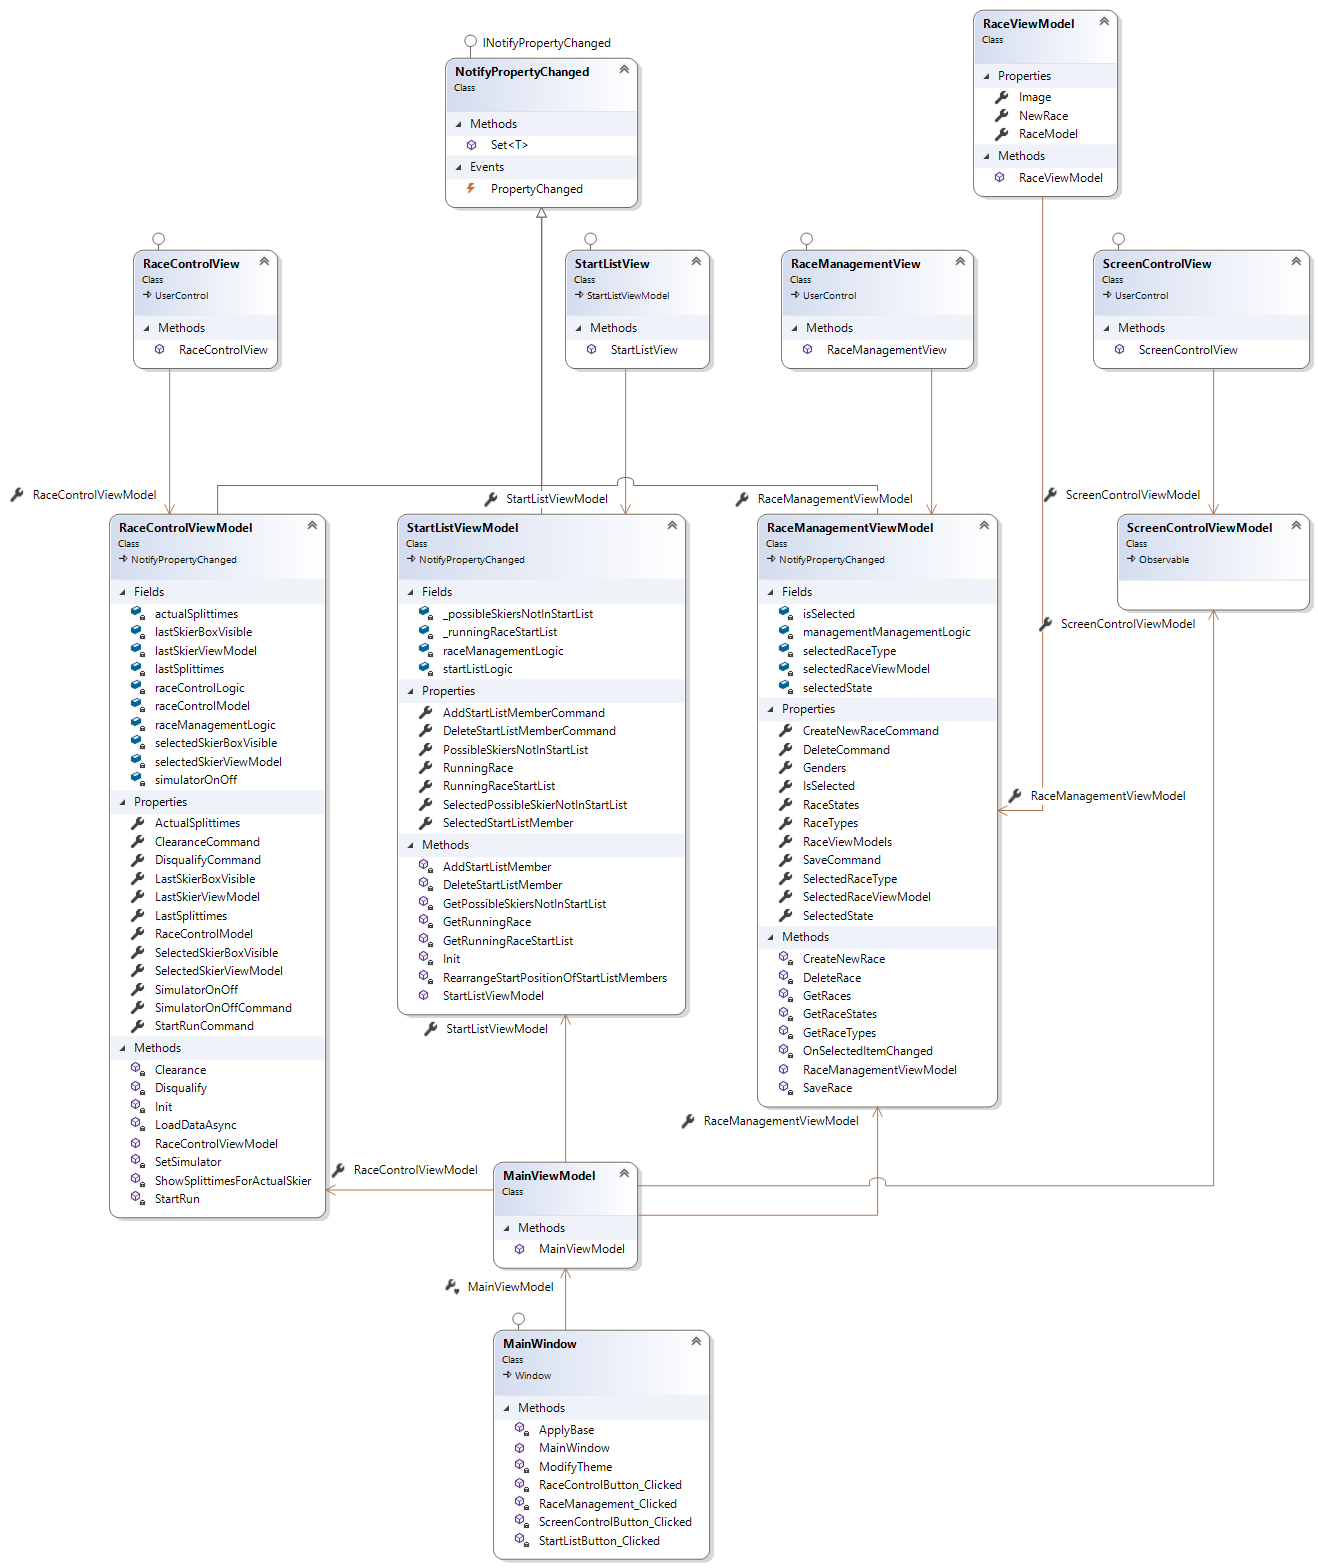
\includegraphics[width=.9\textwidth]{img/RaceControl.png}
	\subsubsection{User Interface}
	
	Damit die optische Komponente einen guten Anstrich bekommt, haben wir uns entschieden Material Design zu verwenden, dieses wurde als Nuget Package hinzugefügt und eingebunden, hierbei haben wir uns für das DarkTheme entschieden. Das UI ist nach dem MVVM Muster gebaut und verwendet dessen Vorteile.\\
	Da der Code sehr umfangreich ist wurde dieser nicht in dieses Dokument eingepflegt.
	
	\newpage
	\subsubsection{Core Logic}
	Um eine Abtrennung der Logik von der Datenbankschicht zu schaffen wurden Interfaces verwendet damit die Datenbankschicht einfach ausgetauscht werden kann. Um die Daten sauber dem UI bereitzustellen wurden Models verwendet um das MVVM Muster umzusetzen.
	\newline
	
	\textbf{IRaceControlLogic}
	\lstinputlisting[language=c++]{../Core.Logic/Interface/IRaceControlLogic.cs}
	\textbf{IRaceManagementLogic}
	\lstinputlisting[language=c++]{../Core.Logic/Interface/IRaceManagementLogic.cs}
	\textbf{IScreenControl}
	\lstinputlisting[language=c++]{../Core.Logic/Interface/IScreenControl.cs}
	\textbf{IStartListLogic}
	\lstinputlisting[language=c++]{../Core.Logic/Interface/IStartListLogic.cs}
	
	\subsection{Verwaltung von Rennen}
	Im Race Management können Rennen hinzugefügt, bearbeitet und gelöscht werden. Ausserdem kann angegeben werden ob das Rennen gerade läuft oder nicht.
	\newline
	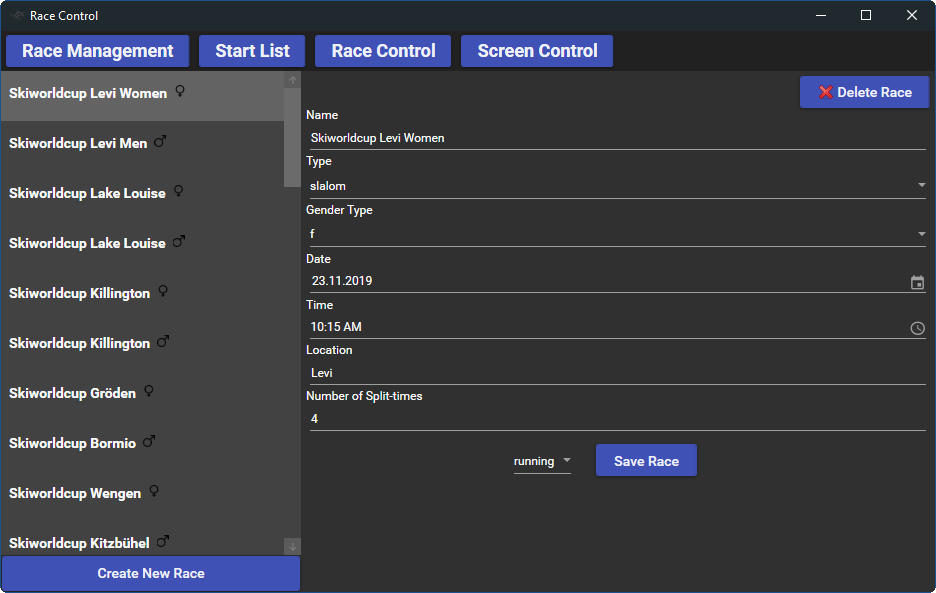
\includegraphics[width=.7\textwidth]{img/ui_raceManagement.png}
	\newline
	
	\subsection{Zuordnung von Rennläuferinnen}
	In Start List werden die Rennläufer bzw. Rennläuferinnen dem gerade laufendem Rennen zugewiesen. Die Rennläufer können auch wieder aus der Startliste entfernt werden. Das Geschlecht wird bei der Auswahl berücksichtigt.
	\newline
	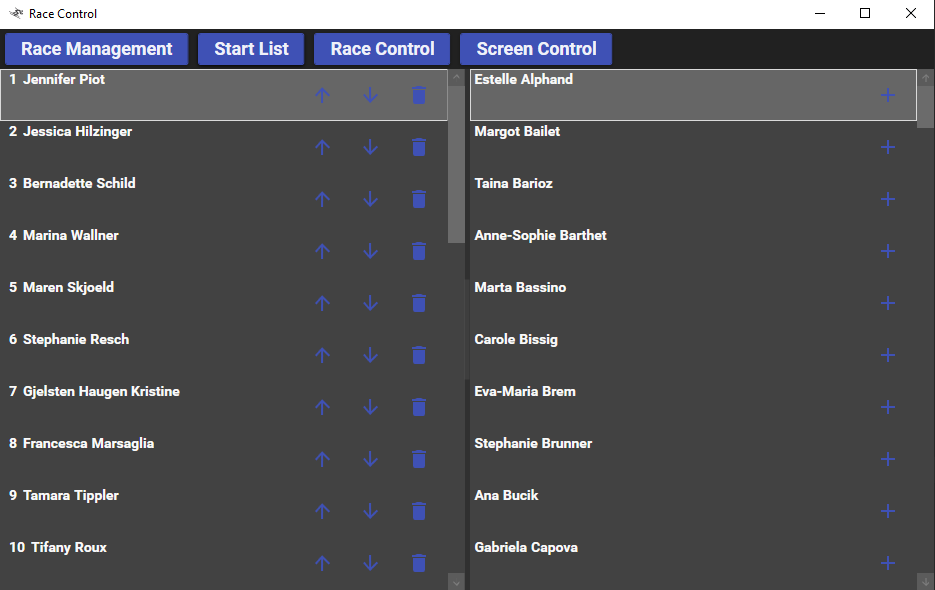
\includegraphics[width=.7\textwidth]{img/ui_startList.png}
	\newline
	
	\subsection{Steuerung des Rennablaufs}
	In Race Control wird der Rennablauf des aktuell laufendem Rennen verwaltet. Der Simulator kann ein und ausgeschaltet werden. Es werden die Zwischenzeiten der bereits gefahrenen Rennläufer dargestellt. Für den aktuell fahrenden Rennläufer werden die Zwischenzeiten in Echtzeit angezeigt. Ein Rennläufer kann freigegeben und disqualifiziert werden. Es muss explizit angegeben werden, dass der Rennläufer im Ziel ist.
	\newline
	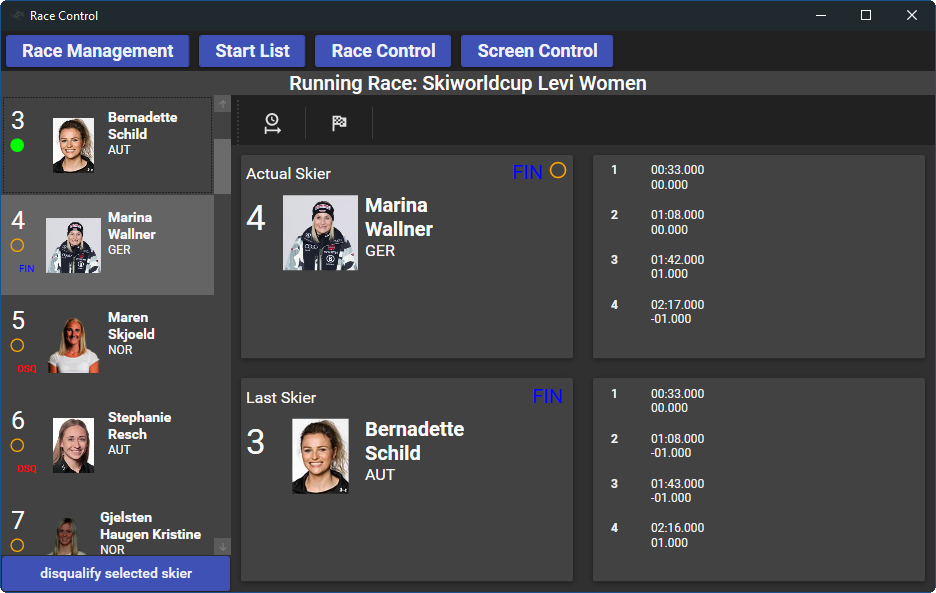
\includegraphics[width=.7\textwidth]{img/ui_raceControl.png}
	\newline
	
	
	\subsection{Steuerung der Anzeigetafel}
	Die Steuerung der Anzeigetafel wurde aus Zeitgründen nicht mehr umgesetzt.
	
	\subsection{Kapselung der Logik}
	Um die Logik weitestgehend zu Kapseln enthält RaceControl selbst wenig Logik. Es greift auf die Komponente Hurace.Logic zu welches wiederum auf die Hurace.Core und Hurace.DAL Komponenten zugreift.
	
	\subsection{UnitTests}
	Zum Testen der Logik wurde das Mocking Framework Moq verwendet, dieses bietet die Möglichkeit die Datenbankschickt mit gemockten Daten zu abstrahieren wenn man diese mittels Interfaces implementiert hat.
	
	Beispieltests:
	\textbf{IStartListLogic}
	\lstinputlisting[language=c++]{../HuraceTest/RaceManagementLogicTests.cs}
	
	
	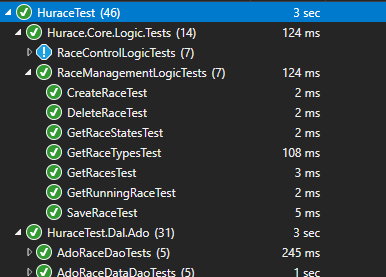
\includegraphics[width=.7\textwidth]{img/UnitTests2.png}

	\newpage
	
	\section{Hurace.Api}
	Bei der Api handelt es sich um ein ASP.NET Core Projekt. Es handelt sich um eine REST Api. Die Api wurde vor Hurace.Web entwickelt und diente somit als Vorlage. Durch entsprechende Attribute in den Controllern konnte eine OpenApi-Spezifikation für die Api erstellt werden. Über das Tool NSwag von Microsoft wurden über die OpenApi-Spezifikation die TypeScript Clients für das Hurace.Web erstellt. Die einzelnen Controller mit ihren Endpunkten wurden entsprechend der Aufgaben für das Hurace.Web Projekt entwickelt. Die benötigten Dto`s wurden erstellt. Da die Id eines Skiers beim erstellen nicht bekannt ist, gibt es für eingehende Skier ein anderes Dto`s als für ausgehende. Zur Unterscheidung befindet sich im Namen entweder 'In' (für eingehend) oder 'Out'(für ausgehend). 
	\subsection{Swagger}
	Swagger wurde dem Container als Service hinzugefügt um sich die Endpunkte im Browser ansehen zu können und die Clients generieren zu können.
	\subsubsection{Endpunkte}
	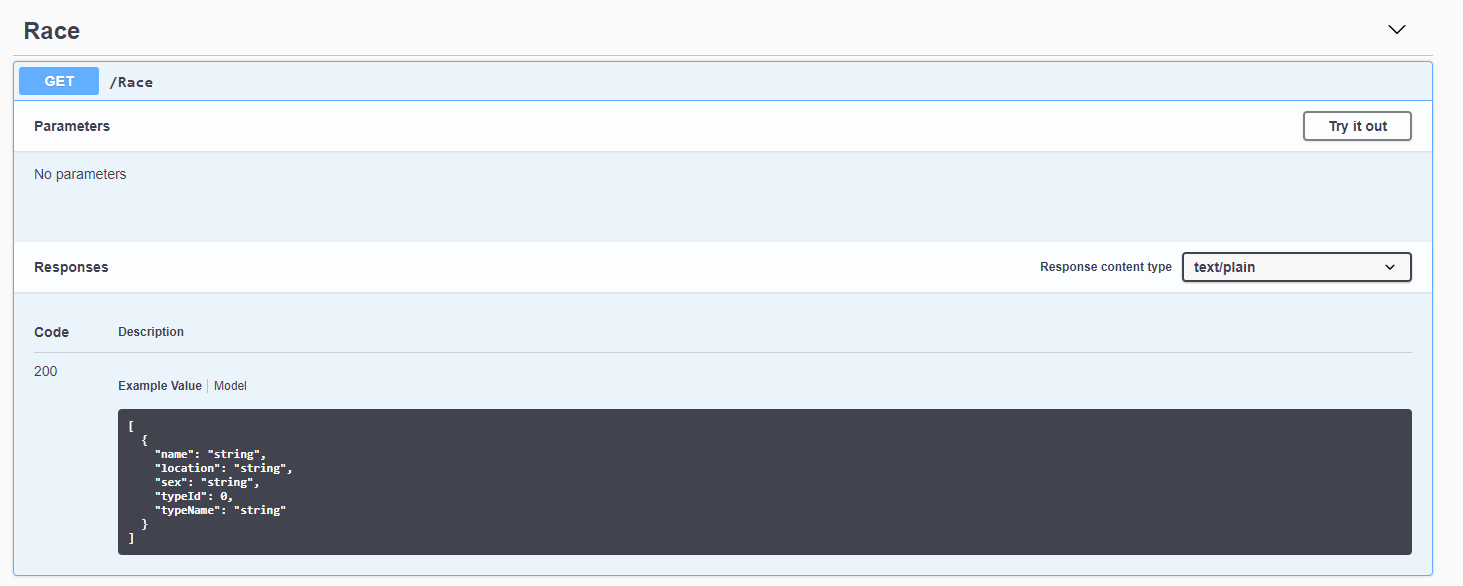
\includegraphics[width=.7\textwidth]{img/Controller_race.png}
	\newline
	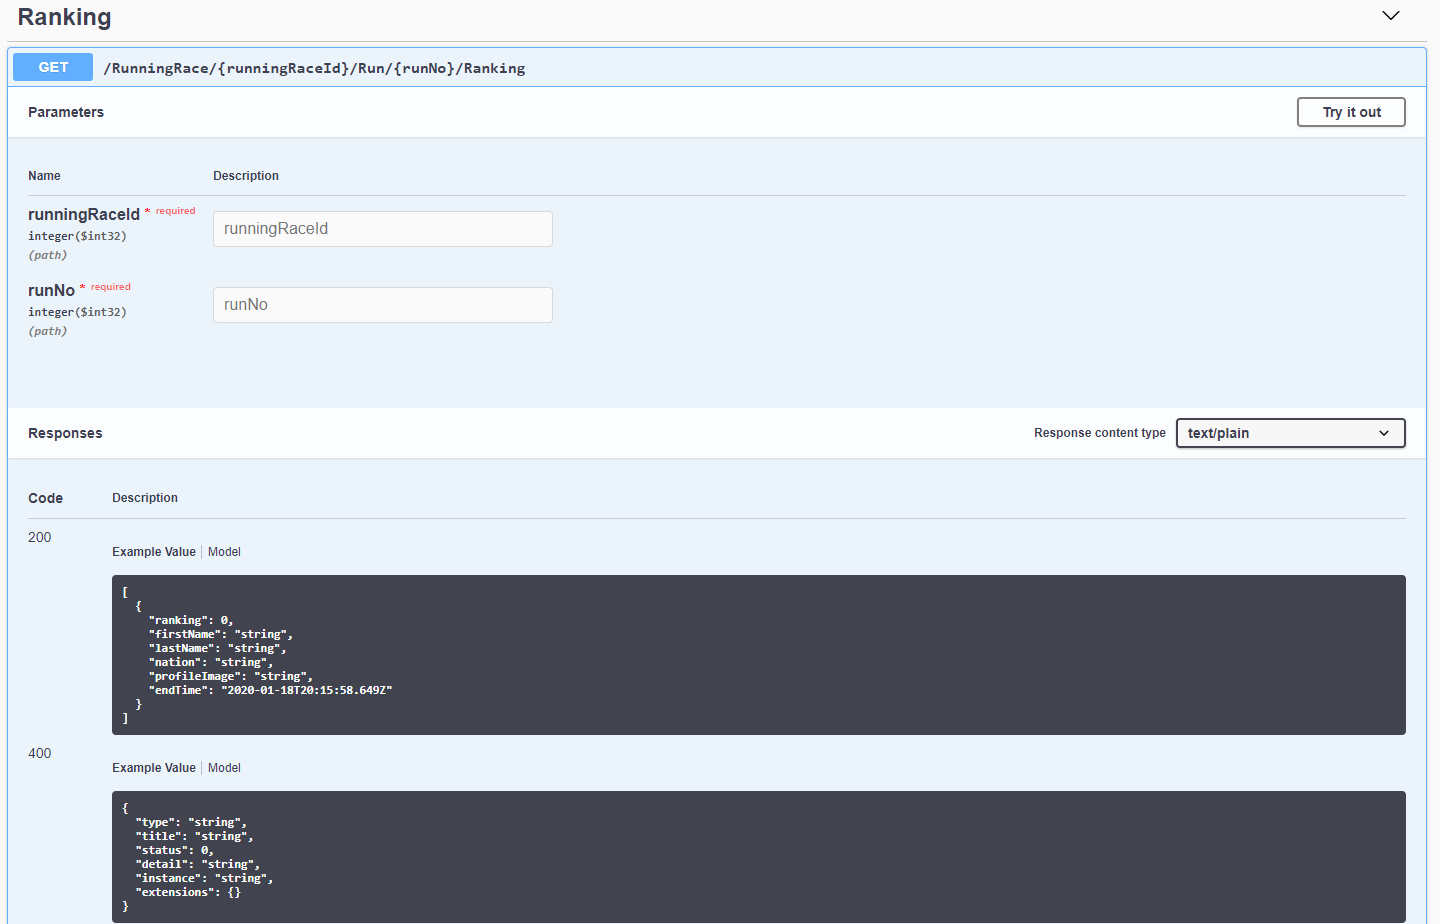
\includegraphics[width=.7\textwidth]{img/Controller_ranking_1.png}
	\newline
	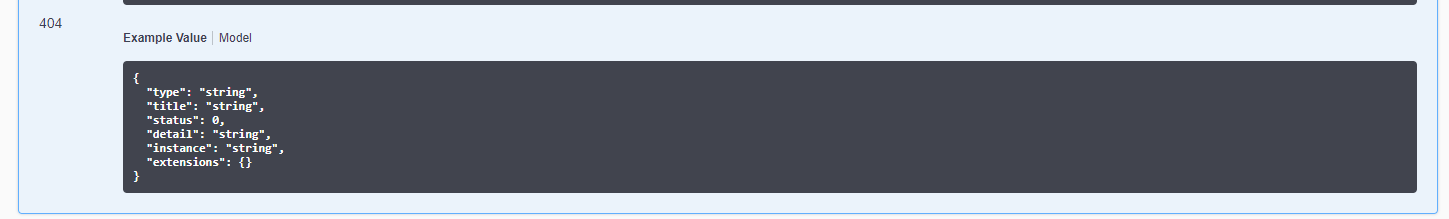
\includegraphics[width=.7\textwidth]{img/Controller_ranking_2.png}
	\newline
	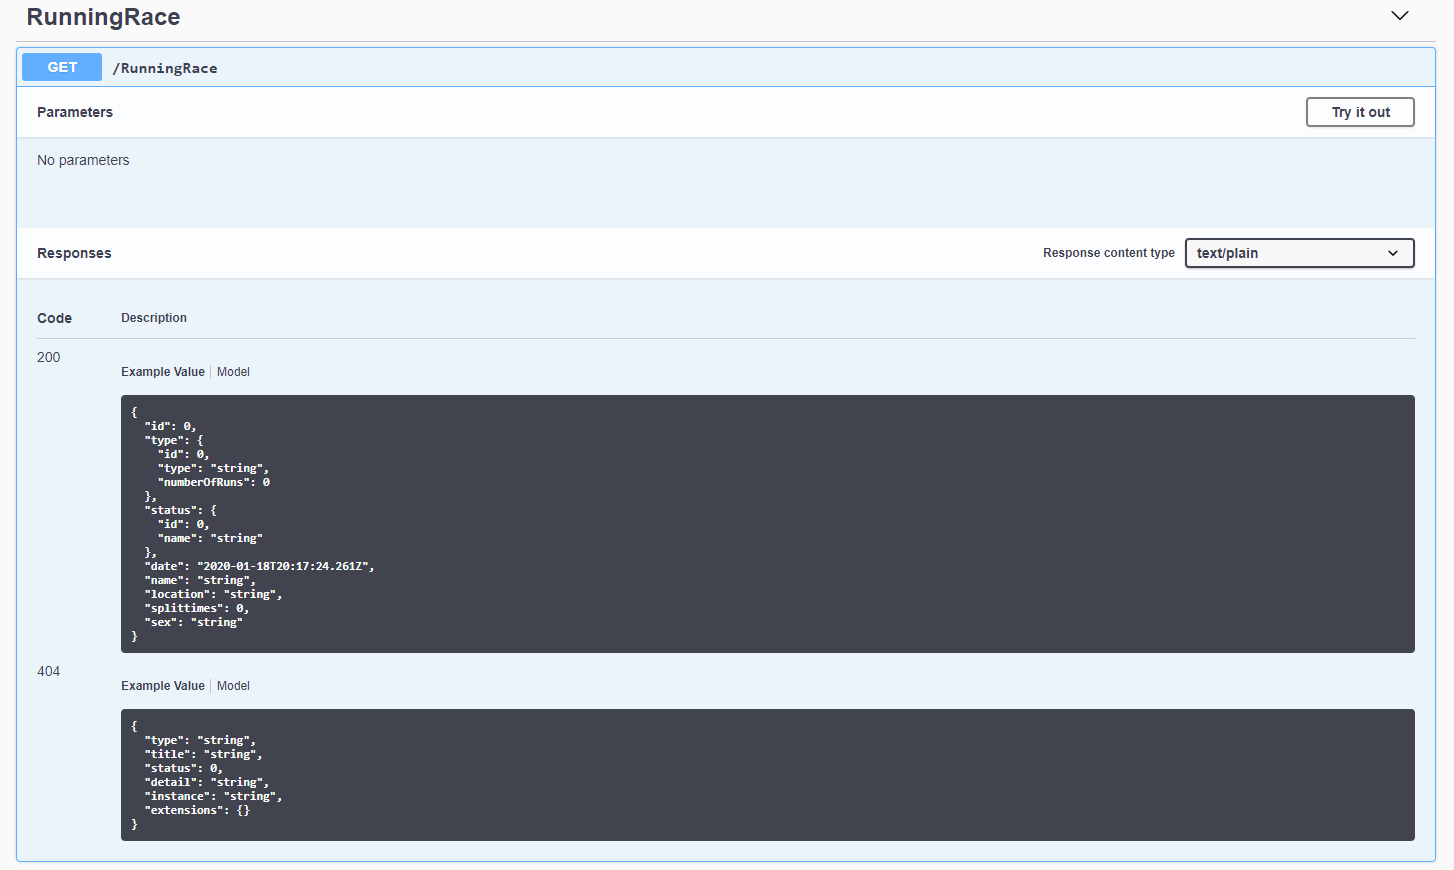
\includegraphics[width=.7\textwidth]{img/Controller_runningRace_get.png}
	\newline
	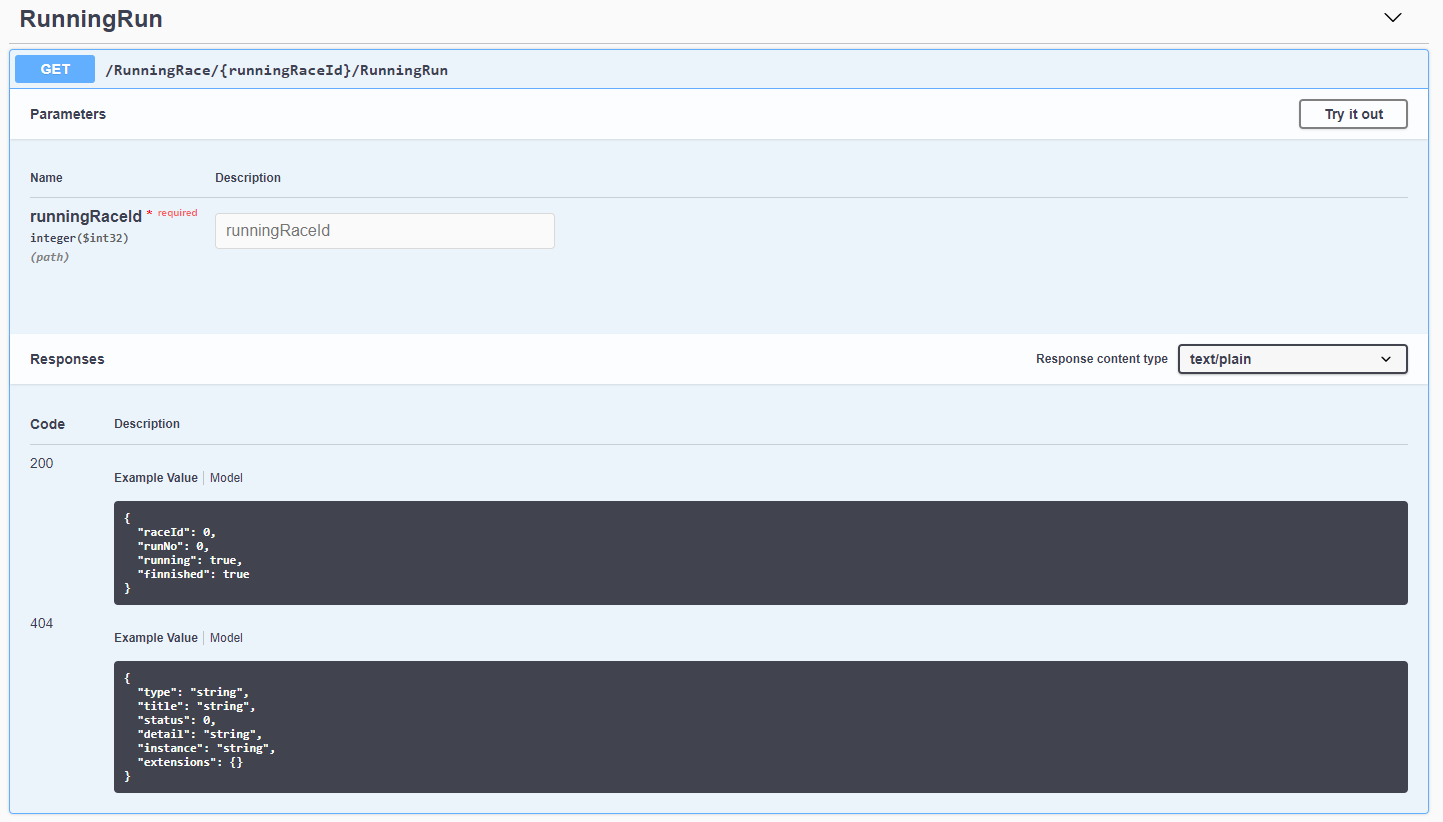
\includegraphics[width=.7\textwidth]{img/Controller_runningRun_get.png}
	\newline	
	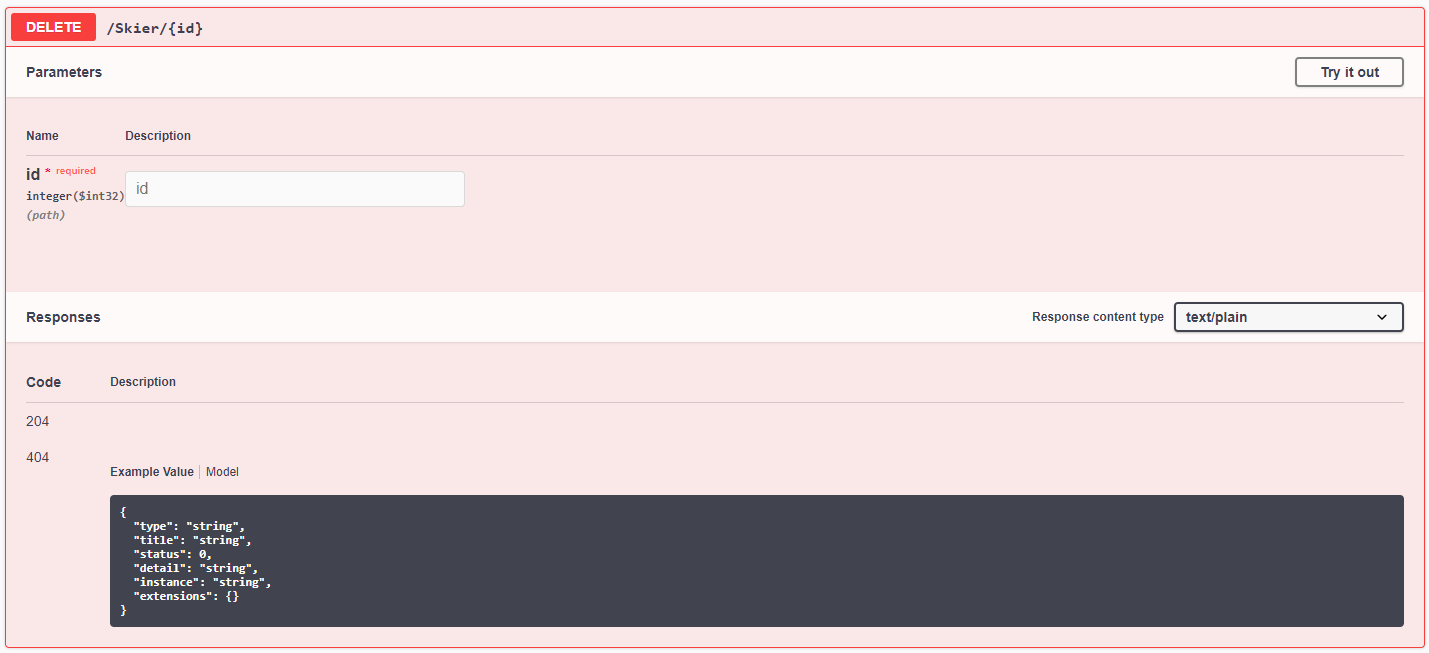
\includegraphics[width=.7\textwidth]{img/Controller_skier_delete.png}
	\newline	
	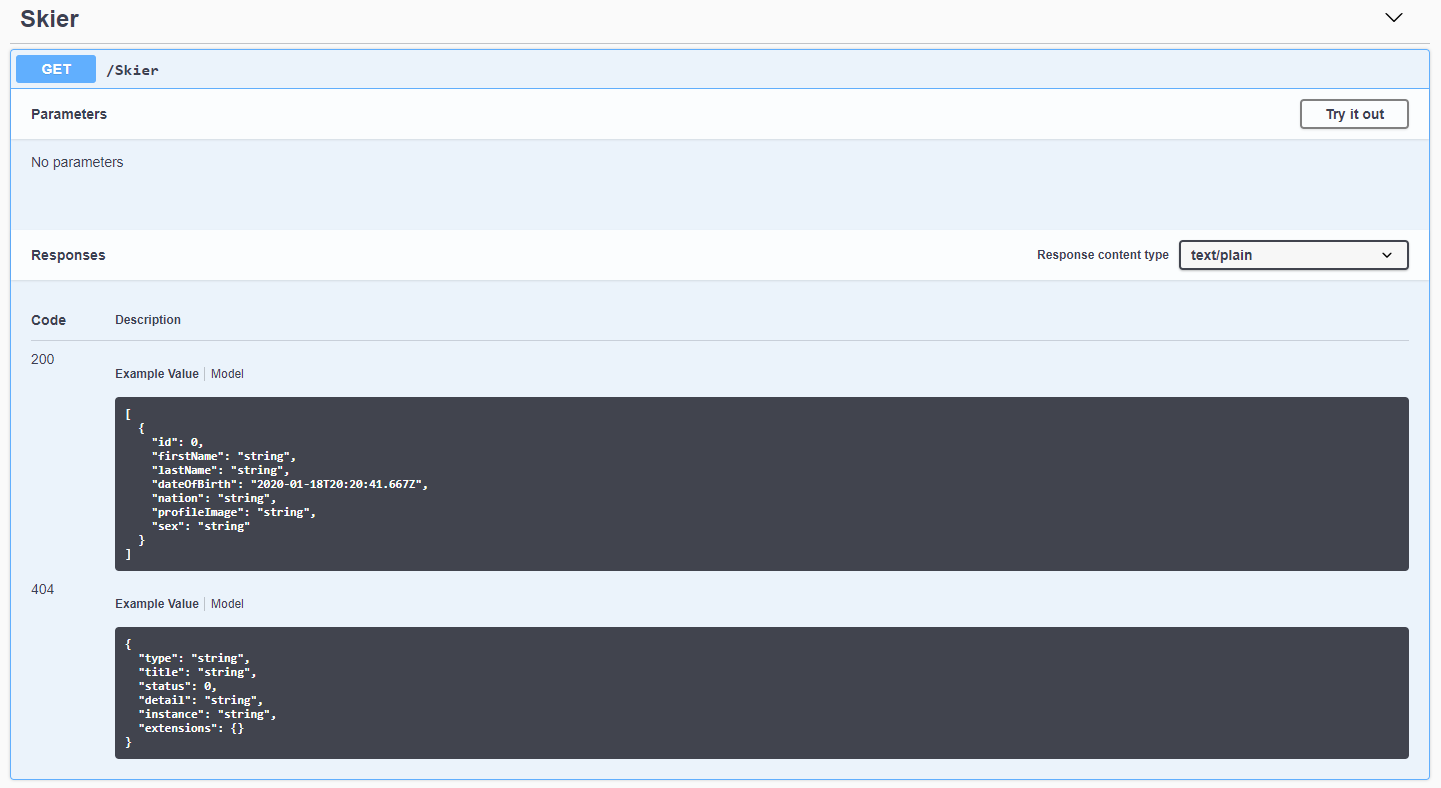
\includegraphics[width=.7\textwidth]{img/Controller_skier_get_all.png}
	\newline	
	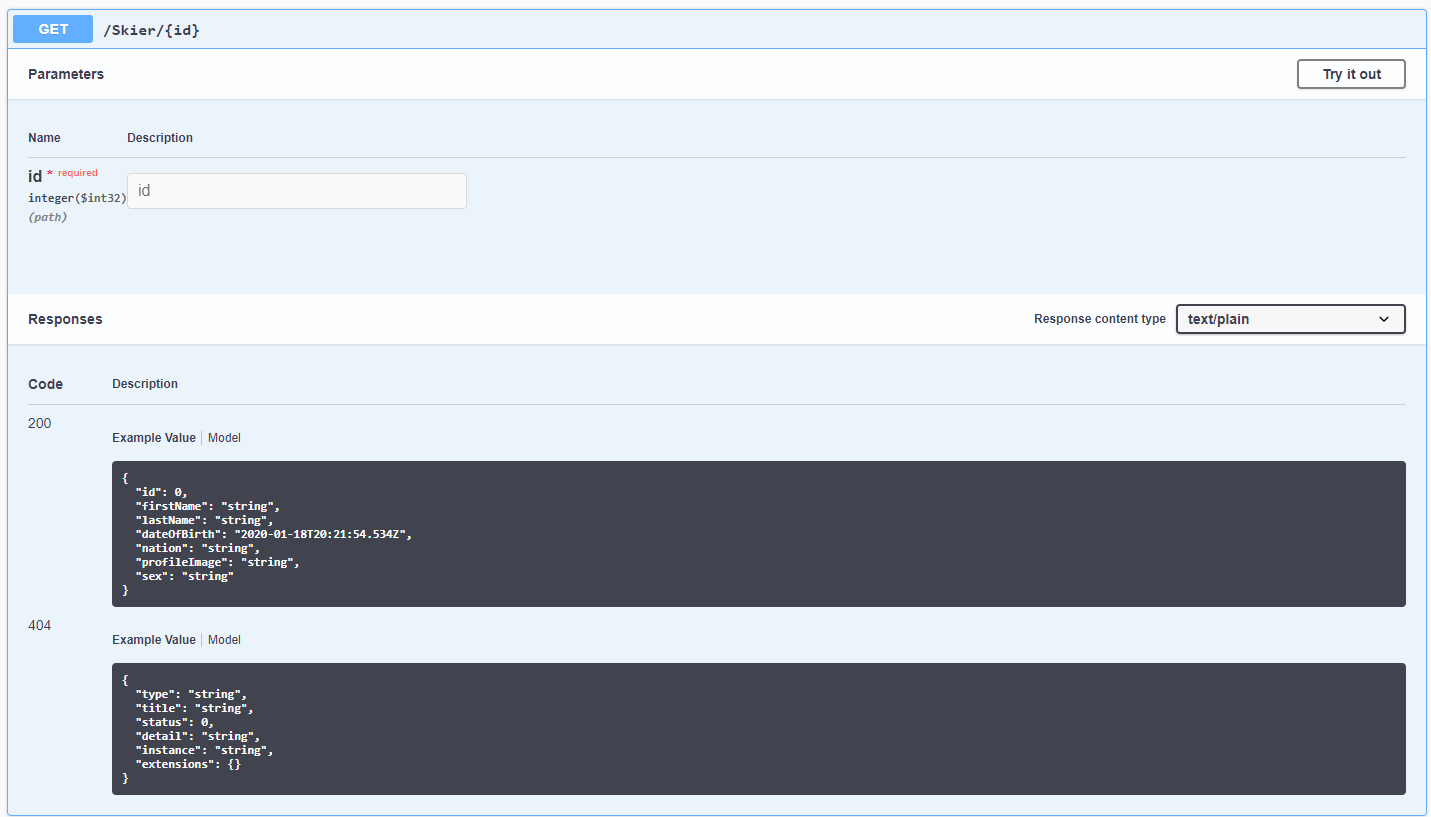
\includegraphics[width=.7\textwidth]{img/Controller_skier_get_byId.png}
	\newline	
	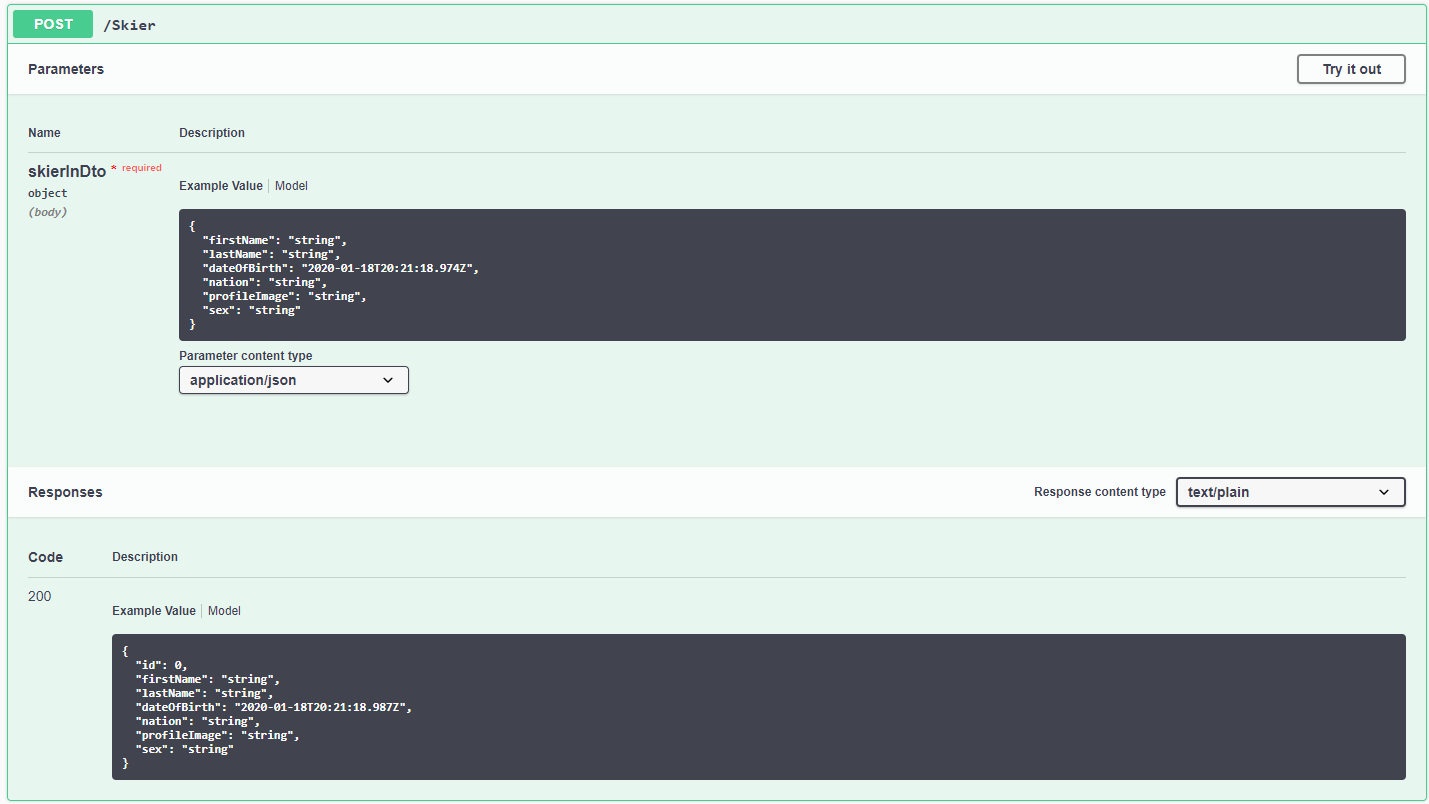
\includegraphics[width=.7\textwidth]{img/Controller_skier_post.png}
	\newline	
	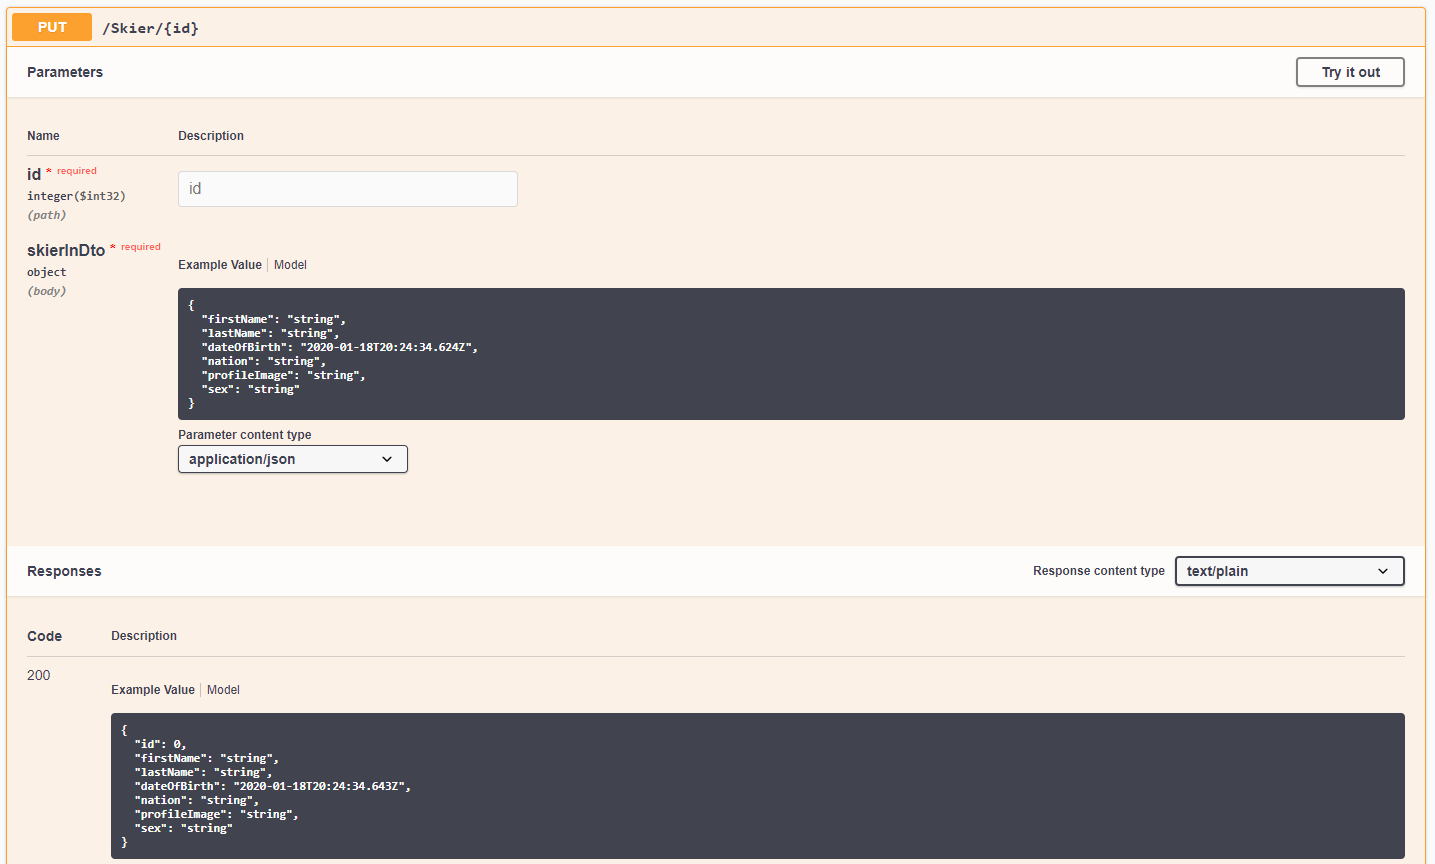
\includegraphics[width=.7\textwidth]{img/Controller_skier_put_1.png}
	\newline	
	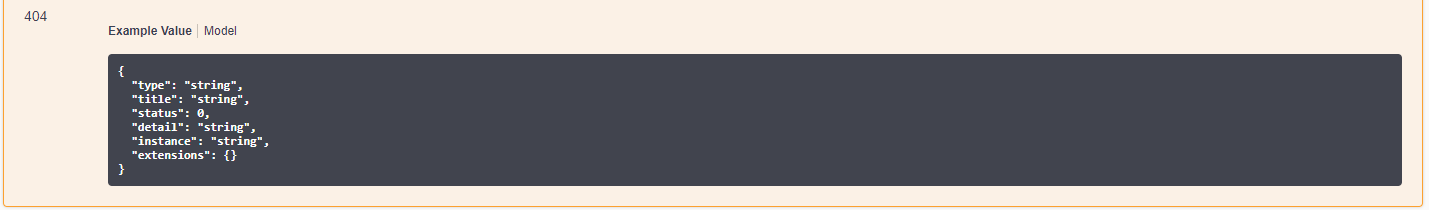
\includegraphics[width=.7\textwidth]{img/Controller_skier_put_2.png}
	\newline	
	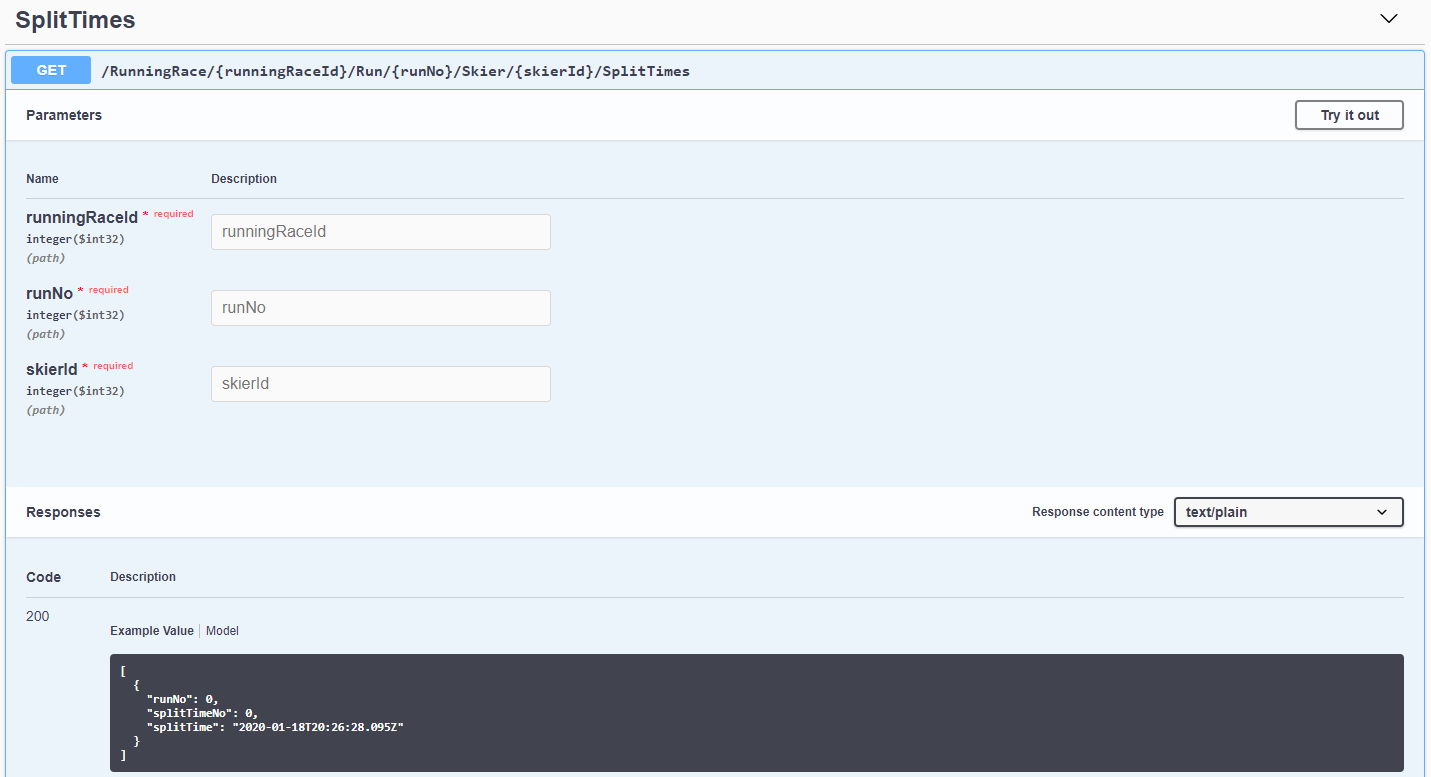
\includegraphics[width=.7\textwidth]{img/Controller_splitTimes_get_1.png}
	\newline
	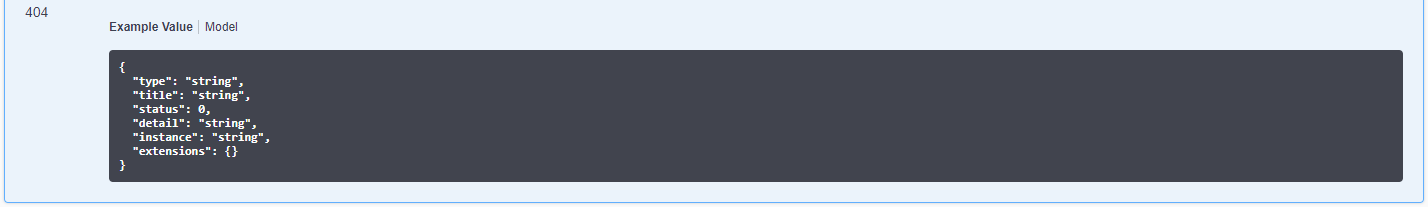
\includegraphics[width=.7\textwidth]{img/Controller_splitTimes_get_2.png}
	\newline
	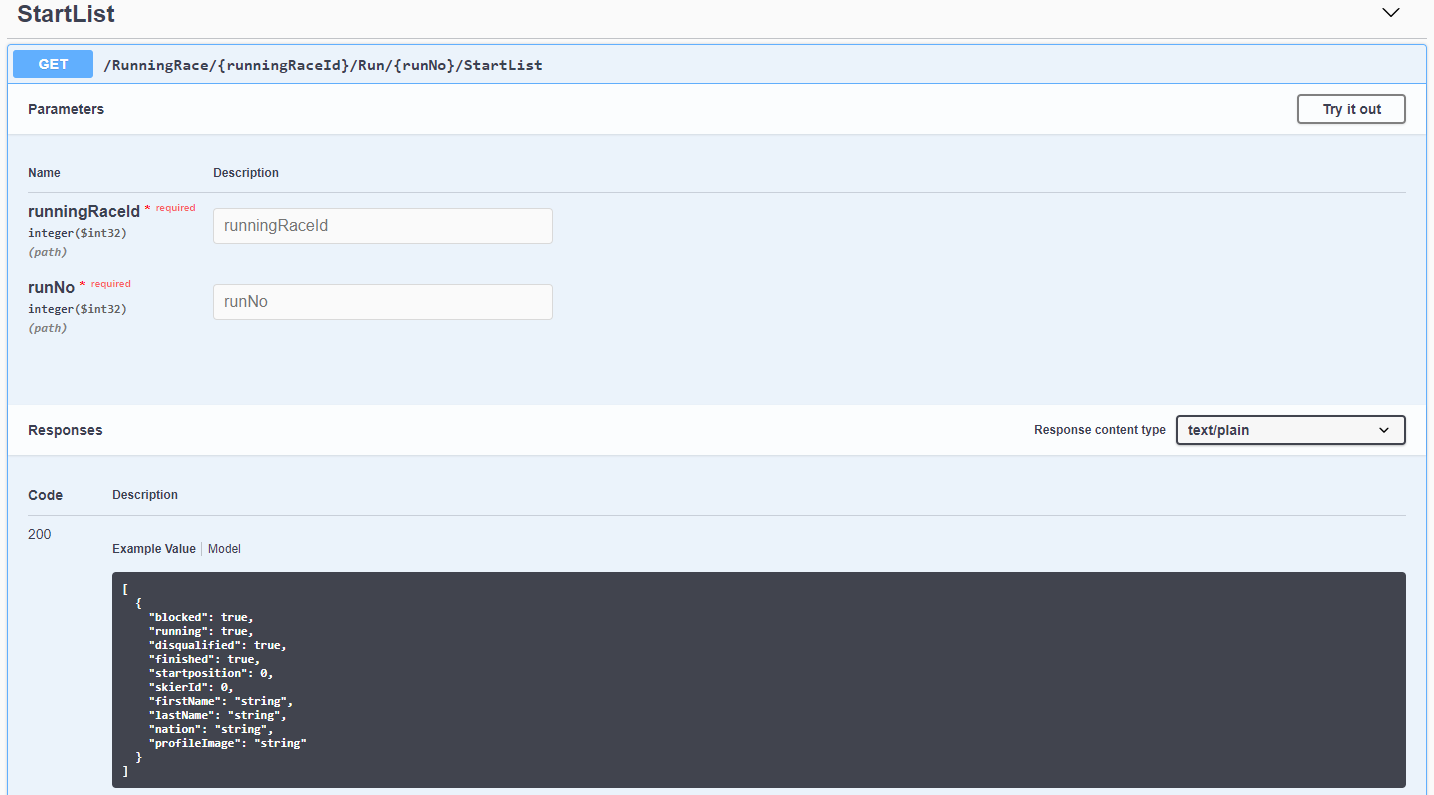
\includegraphics[width=.7\textwidth]{img/Controller_startList_get_1.png}
	\newline
	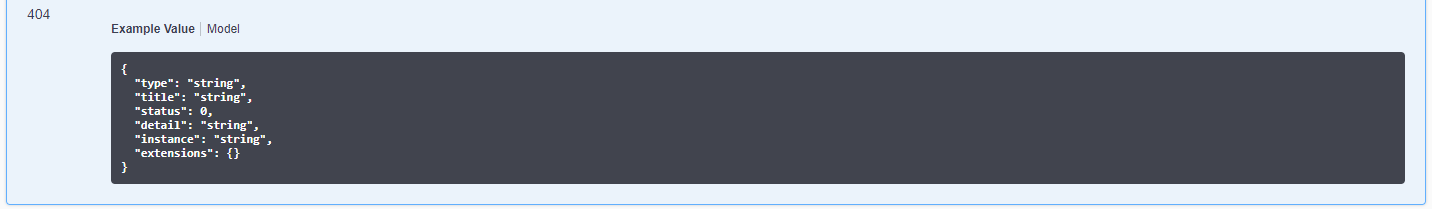
\includegraphics[width=.7\textwidth]{img/Controller_startList_get_2.png}
	\newline
	\subsubsection{Dto`s}
	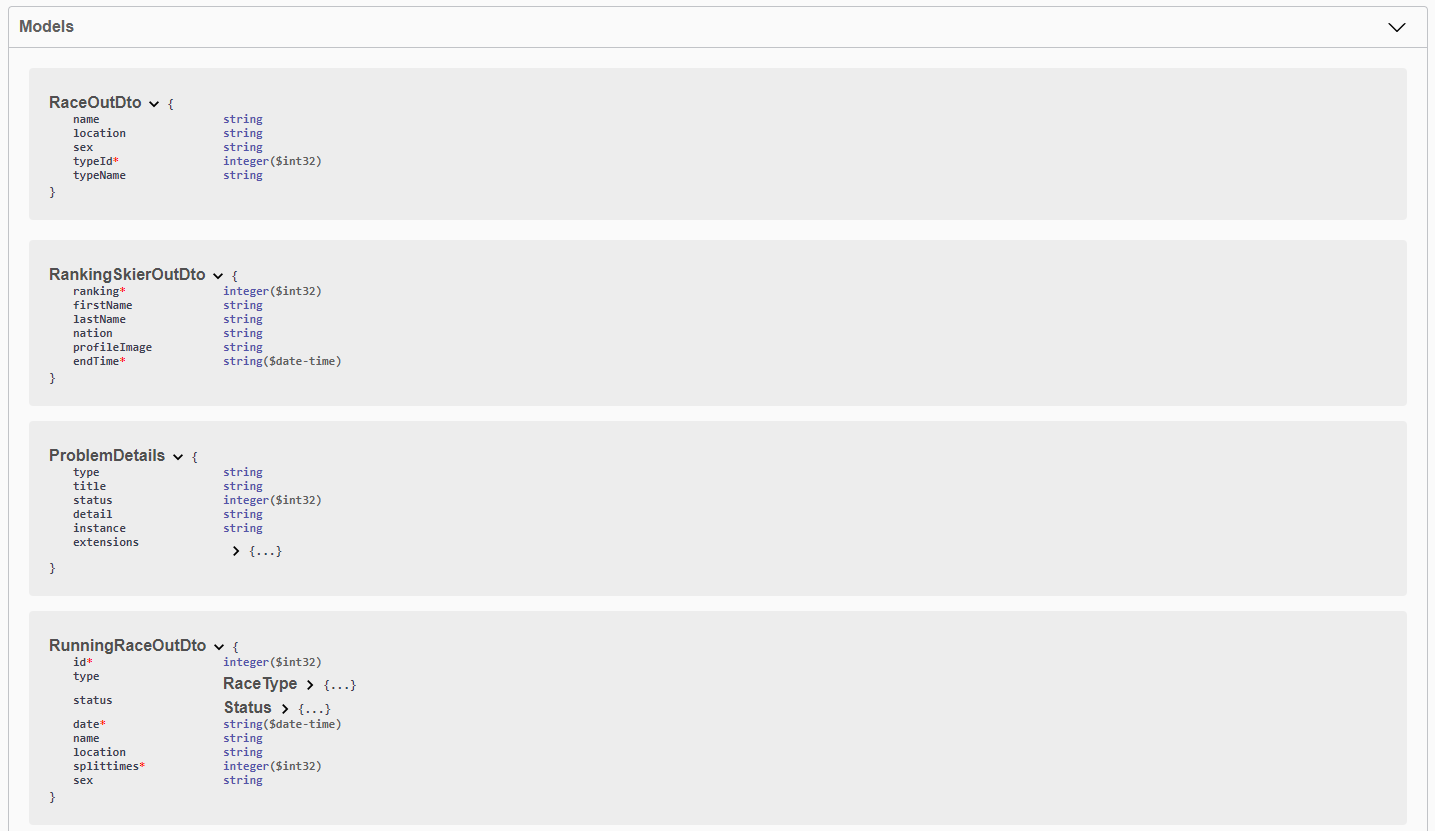
\includegraphics[width=.7\textwidth]{img/Models_1.png}
	\newline		
	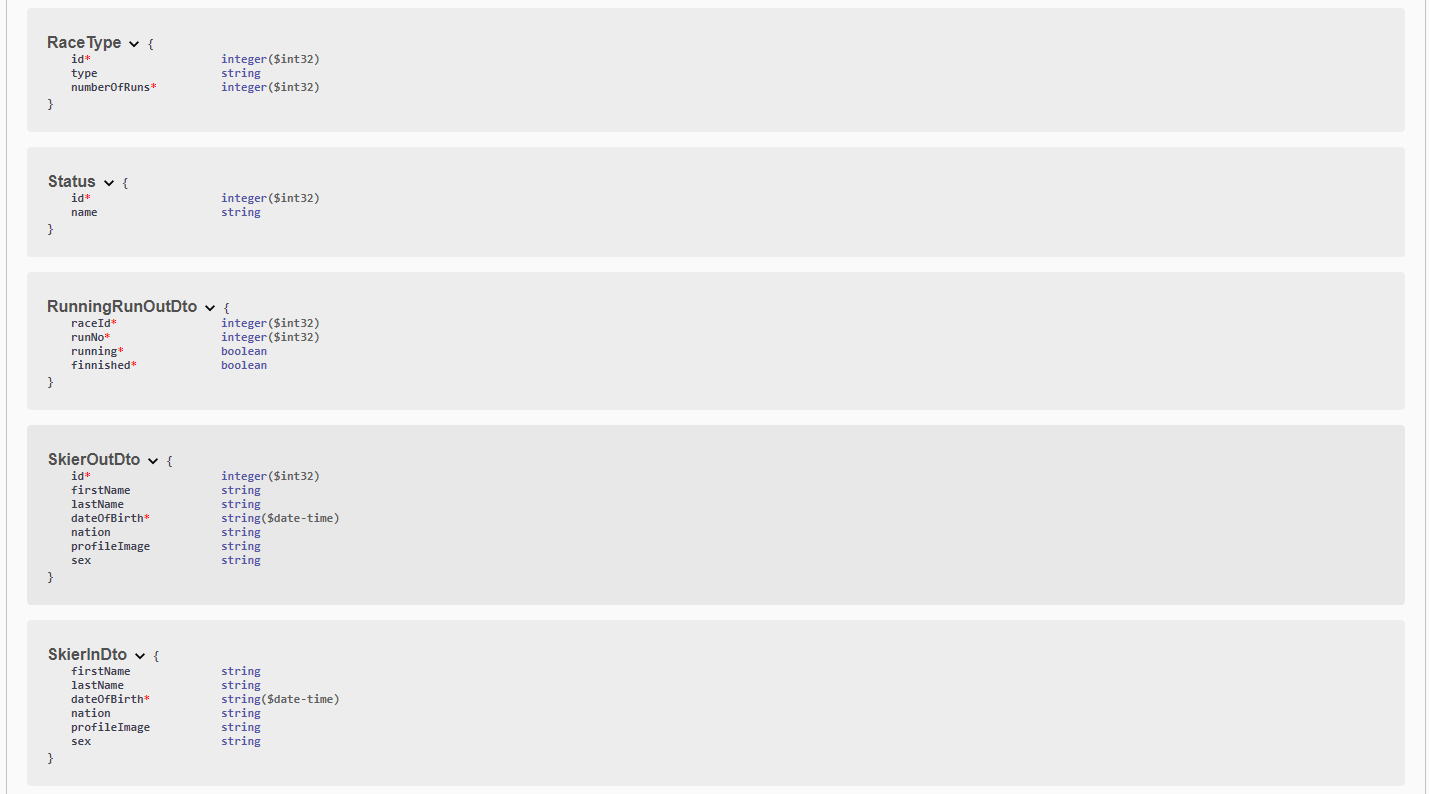
\includegraphics[width=.7\textwidth]{img/Models_2.png}
	\newline		
	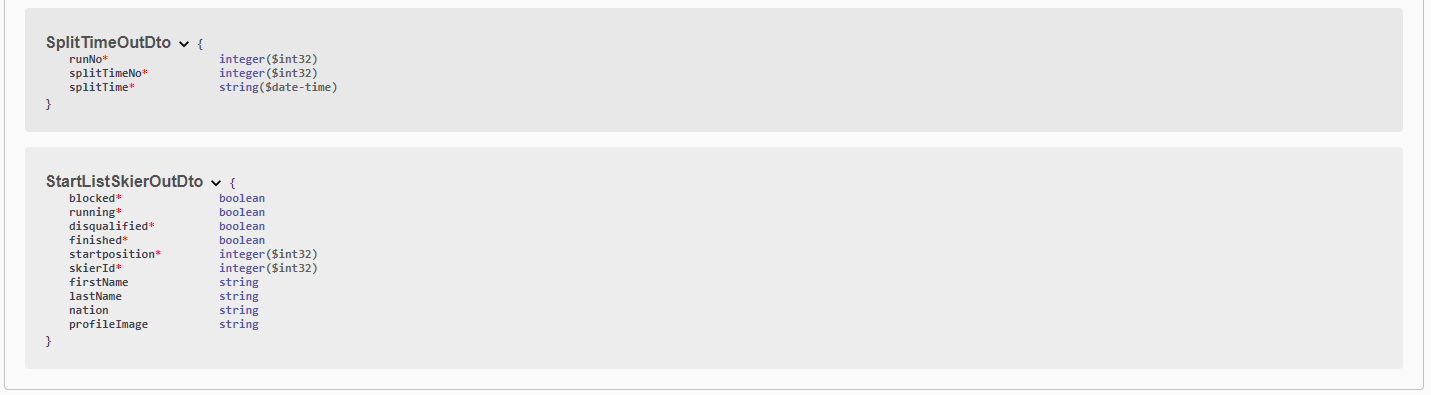
\includegraphics[width=.7\textwidth]{img/Models_3.png}
	\newline		
	\subsubsection{Controller}
	Als Beispiel wird hier der SkierController angeführt. Die Rückgabewerte sind immer in ein ActionResult eingebettet. Dadurch sind einfach lesbare Rückgabefunktionen für verschiedene StatusCodes möglich. Die Controller selbst greifen auf die Dao-Klassen von Core.DAL zu.
	\textbf{IRaceControlLogic}
	\lstinputlisting[language=c++]{../Api/Controllers/SkierController.cs}
	\subsubsection{Dto`s}
	Wie schon beschrieben gibt es beim Skier ein 'In' Dto und ein 'Out' Dto.
	\lstinputlisting[language=c++]{../Api/Dtos/In/SkierInDto.cs}
	\lstinputlisting[language=c++]{../Api/Dtos/Out/SkierOutDto.cs}
	\subsection{CORS}
	Um die Api für den WebClient zugänglich zu machen wird CORS aktiviert. Der Einfachheit halber wurde CORS für alle Domänen und alle Header weitestgehend aktiviert.
	\lstinputlisting[language=c++]{../Api/Startup.cs}
	
	\section{Hurace.Simulator}

	\subsection{Simulation der Zeitnehmung}
	Der Simulator ist in eine eigene Klasse im RaceControl und bekommt vom RaceControl die Aktivierung, wenn dieser aktiv geschalten wurde und ein Skiläufer nicht mehr geblockt ist dann startet der Simulator automatisch den Lauf des Rennläufers. Dieser ruft dann die Methode auf um eine neue Zwischenzeit anzulegen. 
	Die Logik vom RaceControl kümmert sich dann darum um zu entscheiden ob es die erste Zwischenzeit war oder die letzte um den Lauf zu beenden. Ist ein Läufer vom Steuermann disqualifiziert worden so werden keine weiteren Zwischenzeiten von dieser Instanz des Simulators akzeptiert.
	
	\subsection{Benutzerinteraktion}
	Der Simulator kann mit einem Switch im RaceControl aktiviert werden, je nach Renntyp und Durchgang generiert er andere Zeiten.
	
	
\end{document}